\documentclass[alsotrans]{beamerswitch}
\usepackage{sdp}

\title{Дървета}

\date{2 декември 2019 г.}

\titlegraphicx{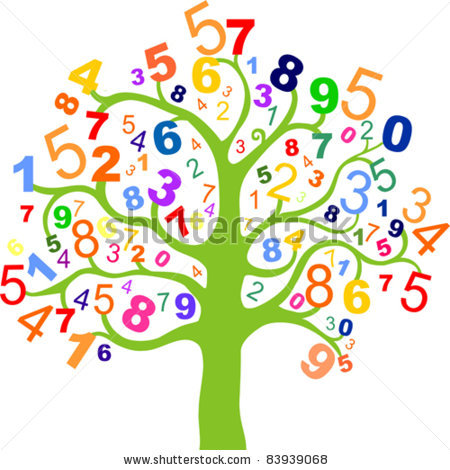
\includegraphics[height=0.25\textheight]{images/tree.jpg}\\
  \imageUntitledAttr{bluebudgie}{https://www.needpix.com/photo/1269899/wordcloud-trees-knowledge-tagcloud-text-cloud-word-info-design}{CC0}}

\forestset{default/.style={baseline,for tree={fill=diagramblue,draw,circle,inner
      sep=0pt,minimum size=4ex,edge=->}}}

\newcommand{\sampletree}{%
  \begin{forest} default
    [1 [2 [3] [4 [5] [6]] [7] [8]] [9] [10]]
  \end{forest}%
}

\newcommand{\samplebintree}{%
      \begin{forest}
        default
        [a [a$_0$ [a$_{00}$ [a$_{000}$] [,phantom]] [a$_{01}$ [,phantom] [a$_{011}$]]] [a$_1$ [,phantom] [a$_{11}$ [,phantom] [a$_{111}$]]]]
      \end{forest}%
}


\begin{document}

\begin{frame}
  \titlepage
\end{frame}

\section{Коренови дървета}

\begin{frame}
  \frametitle{Пример: кореново дърво}
  \begin{center}
    \sampletree
  \end{center}
\end{frame}

\begin{frame}
  \frametitle{АТД: Дърво}
  Йерархична структура, в която на всеки елемент е съпоставено множество от подчинени елементи.
  \begin{definition}
    Кореново дърво е списък $(X, T_1, \ldots, T_n)$, където
    \begin{itemize}
    \item $X$ е данна (корен)
    \item $T_1, T_2, \ldots, T_n$ са коренови дървета (поддървета)\pause, \alert{$n\geq 0$}
    \end{itemize}
  \end{definition}
  \pause
  Често отъждествяваме кореновите дървета с корените им (\textbf{възли}).\\
  \pause
  Операции:
  \begin{itemize}
  \item \tt{create(x)} --- създаване на дърво с корен $x$
  \item \tt{addChild(t)} --- добавяне на поддърво $t$
  \item \tt{root()} --- достъп до корена
  \item \tt{subtrees()} --- достъп до поддърветата
  \end{itemize}
\end{frame}

\begin{frame}
  \frametitle{Свързано представяне}
  Свързана структура от възли, където всеки възел се състои от:
  \begin{itemize}
  \item стойността на корена
  \item свързан списък от възли, представящи поддърветата (деца)
  \end{itemize}
  % TODO: да се нарисува с TikZ
  \begin{center}
    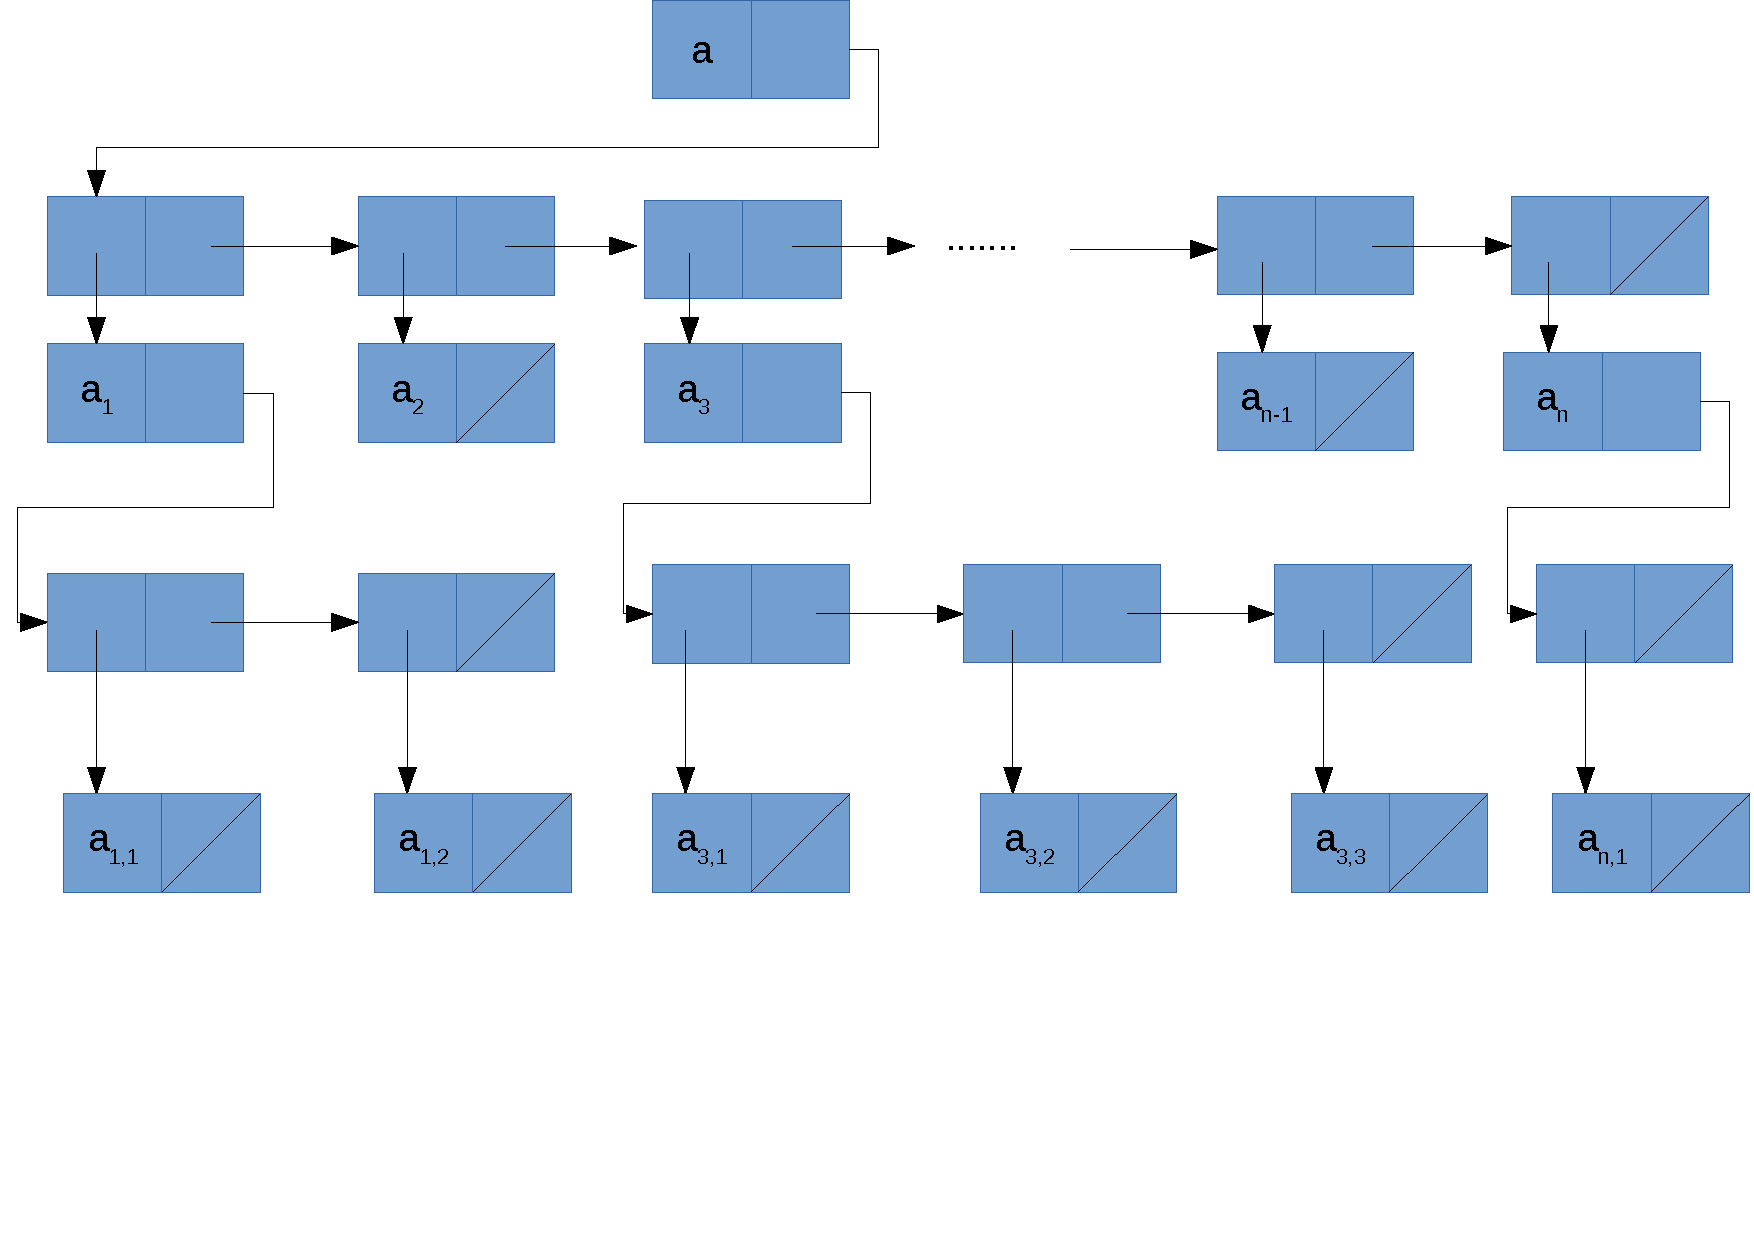
\includegraphics[height=0.65\textheight]{images/mtree.pdf}
  \end{center}
\end{frame}

\begin{frame}
  \frametitle{Последователно представяне}
  Последователност от тройки (корен, най-ляво дете, десен брат)\\[2ex]
  \begin{center}
    \begin{tabular}{|r*{10}{|c}|}
      \cline{2-11}
      \multicolumn1{c|}{} &
      0    &    1    &    2    &    3    &    4    &    5    &    6    &    7    &    8    & \ldots\\
      \hline
      корен &
      a    &  a$_1$  & a$_{1,1}$&  a$_2$  &a$_{1,2}$ &  a$_3$  &a$_{3,1}$&a$_{3,2}$ &a$_{3,3}$ & \ldots\\
      \hline
      най-ляво дете &
      1    &    2    &   -1    &    -1   &   -1    &    6    &   -1    &   -1    &   -1    &  \ldots\\
      \hline
      десен брат &
      -1   &    3    &    4    &    5    &   -1    &    9    &    7    &    8    &   -1    &  \ldots\\
      \hline
    \end{tabular}
  \end{center}
\end{frame}

\begin{frame}
  \frametitle{Дефиниции за дърво}
  \begin{columns}
    \begin{column}{0.65\textwidth}
      \begin{itemize}
      \item \textbf{дете} --- коренов възел на поддърво
      \item \textbf{родител} --- възел, сред чиито деца е коренът
      \item \textbf{листо} --- възел без деца
      \item \textbf{път} --- редица от възли, в която всеки следващ дете на предходния
      \item \textbf{разстояние} --- дължина на пътя от корена до даден възел
      \item \textbf{ниво} --- множество от възлите на еднакво разстояние
      \item \textbf{височина (дълбочина)} --- максималното разстояние в дървото
      \item \textbf{широчина (разклоненост)} --- максималният брой деца на възел
      \end{itemize}
    \end{column}
    \begin{column}{0.35\textwidth}
      \sampletree
    \end{column}
  \end{columns}
\end{frame}

\begin{frame}
  \frametitle{Схеми за обхождане}
  \begin{columns}
    \begin{column}{0.65\textwidth}
      \begin{itemize}
      \item префиксно обхождане
        \begin{itemize}
        \item първо посещаваме корена
        \item след това обхождаме децата
          \pause
        \item 1, 2, 3, 4, 5, 6, 7, 8, 9, 10
        \end{itemize}
        \pause
      \item постфиксно обхождане
        \begin{itemize}
        \item първо обхождаме децата
        \item накрая посещаваме корена
          \pause
        \item 3, 5, 6, 4, 7, 8, 2, 9, 10, 1
        \end{itemize}
      \end{itemize}
    \end{column}
    \onslide<1->
    \begin{column}{0.35\textwidth}
      \sampletree
    \end{column}
  \end{columns}
\end{frame}

\section{Двоични дървета}

\begin{frame}
  \frametitle{Дървета с фиксиран брой поддървета}
  Ако искаме всеки възел на дървото да има един и същ (максимален) брой деца, използваме алтернативна дефиниция
  \pause
  \begin{definition}[$n$-арно дърво]
    \begin{itemize}
    \item $\bot$ (празното дърво)
    \item наредена $n+1$-торка $(X, T_1, \ldots, T_n)$, където
      \begin{itemize}
      \item $X$ е данна (корен)
      \item $T_1, T_2, \ldots, T_n$ са $n$-арни дървета (поддървета)
      \end{itemize}
    \end{itemize}
  \end{definition}
  \pause
  Операции:
  \begin{itemize}
  \item \tt{empty\_tree()} --- създаване на празно дърво
  \item \tt{create\_tree(x,t$_1$,\ldots,t$_n$)} --- създаване на $n$-арно дърво с корен \tt x и поддървета \tt t$_1$, \ldots, \tt t$_n$
  \item \tt{root()} --- достъп до корена
  \item \tt{subtree(i)} --- достъп до \tt i-тото поддърво
  \end{itemize}
\end{frame}

\begin{frame}
  \frametitle{Наредба на поддърветата}
  Дефинициите за коренови дървета и $n$-арни дървета не са еквивалентни!\\[2ex]
  \textbf{Пример:} троични дървета\\[2ex]
  \begin{center}
    \begin{forest}
      default [1 [2] [,phantom] [3]]
    \end{forest}
    $\qquad\neq\qquad$
    \begin{forest}
      default [1 [2] [3] [,phantom]]
    \end{forest}
    $\qquad\neq\qquad$
    \begin{forest}
      default [1 [,phantom] [2] [3]]
    \end{forest}
  \end{center}
  Едно и също кореново дърво може да бъде представено като $n$-арно дърво по няколко различни начина.
\end{frame}

\begin{frame}
  \frametitle{Двоично дърво}
  \begin{columns}[t,onlytextwidth]
    \begin{column}{0.55\textwidth}
      \begin{definition}[двоично дърво]
        \begin{itemize}
        \item $\bot$ (празното дърво)
        \item наредена тройка $(X, L, R)$, където
          \begin{itemize}
          \item $X$ е данна (корен)
          \item $L$ е ляво поддърво
          \item $R$ е дясно поддърво
          \end{itemize}
        \end{itemize}
      \end{definition}
    \end{column}
    \begin{column}{0.45\textwidth}
      \vspace{4ex}
      \samplebintree
    \end{column}
  \end{columns}
\end{frame}

\begin{frame}
  \frametitle{Свързано представяне}
  Свързана структура от тройни кутии\\[2ex]
  % TODO: да се нарисува с TikZ
  \begin{center}
    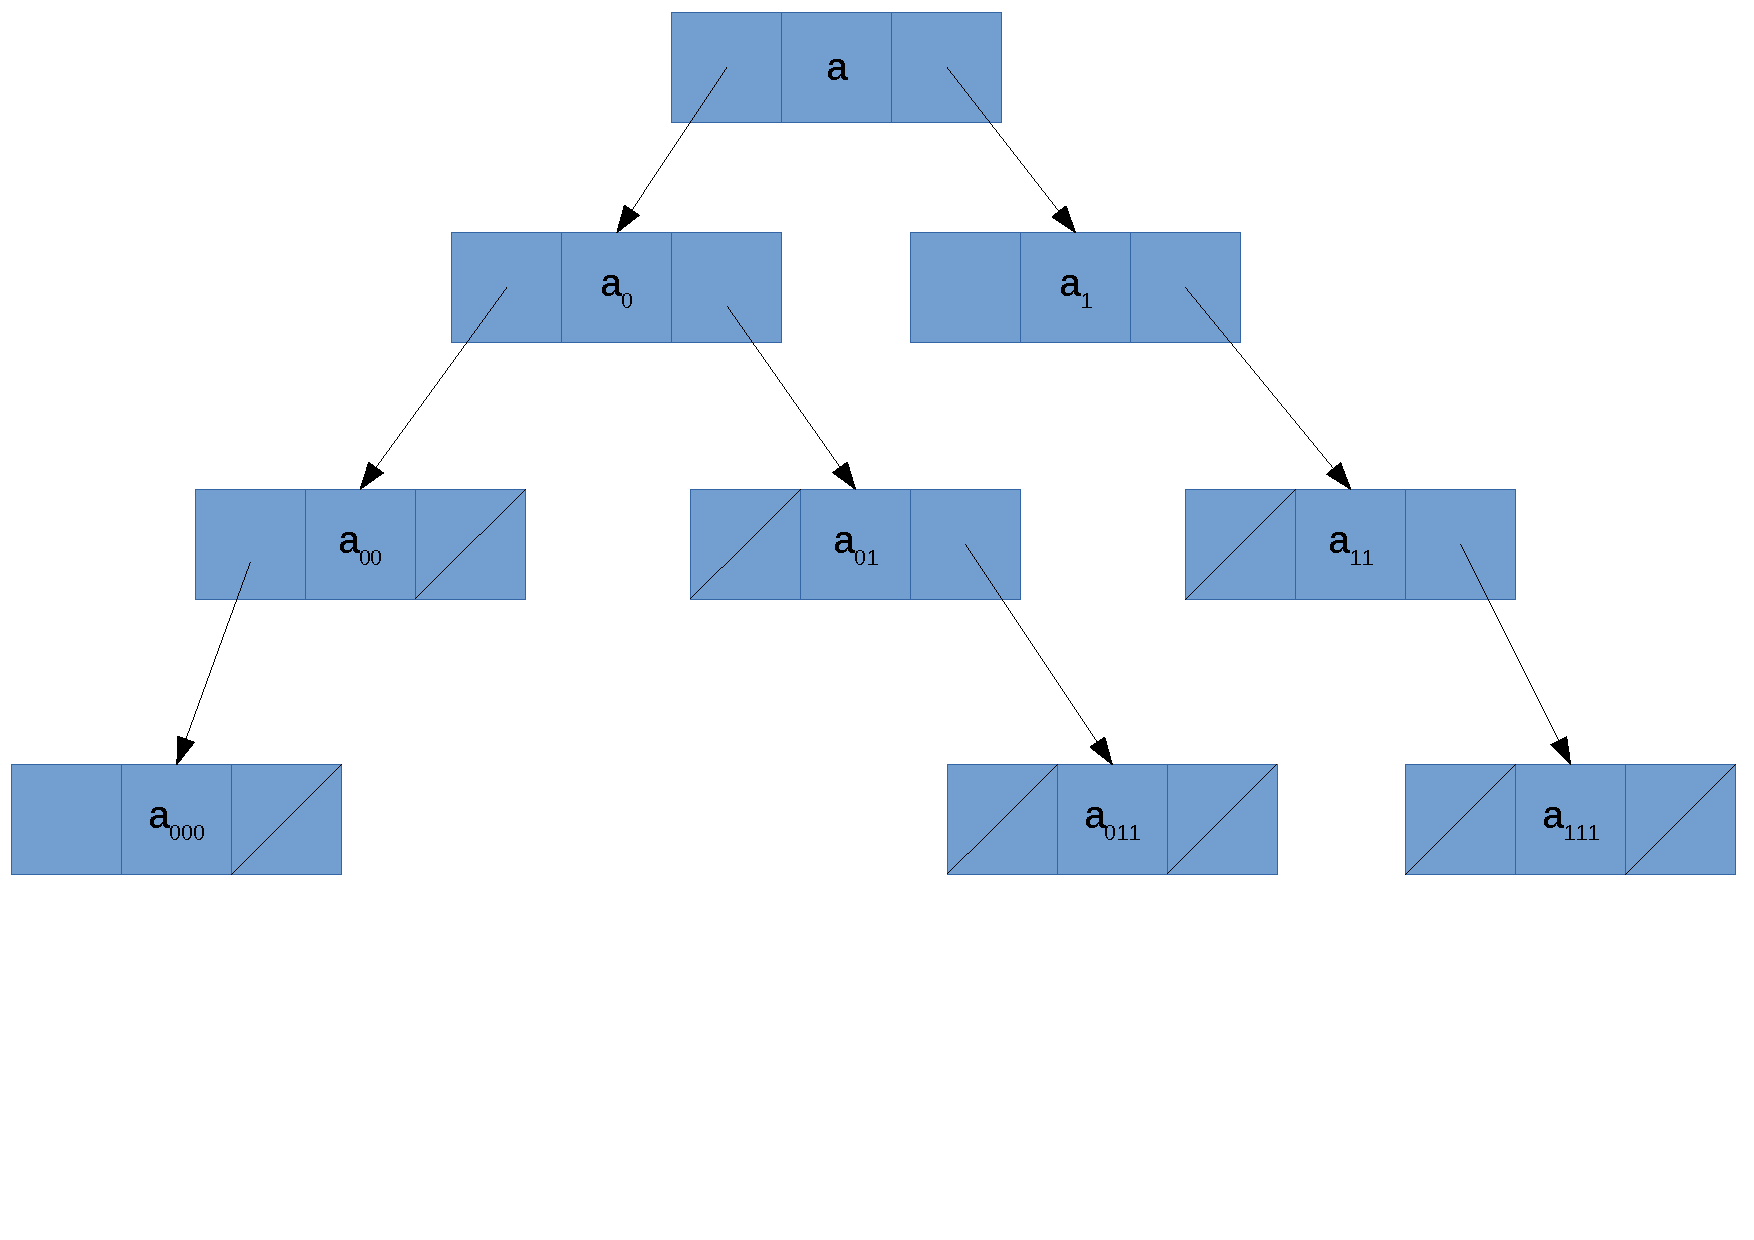
\includegraphics[height=.75\textheight]{images/bintree.pdf}
  \end{center}
\end{frame}

\begin{frame}
  \frametitle{Последователно представяне}
  Последователност от тройки (корен, ляво, дясно)\\[2ex]
  \begin{center}
    \begin{tabular}{|r*{10}{|c}|}
      \cline{2-11}
      \multicolumn1{c|}{} &
      0    &    1    &    2    &    3    &    4    &    5    &    6    &    7    &    8    & \ldots\\
      \hline
      корен &
      a    &  a$_0$  & a$_1$   &a$_{00}$ &a$_{01}$  &a$_{11}$  &a$_{000}$&a$_{011}$ &a$_{111}$ & \ldots\\
      \hline
      ляво дете &
      1    &    3    &   -1    &    6    &   -1    &   -1    &   -1    &   -1    &   -1    &  \ldots\\
      \hline
      дясно дете &
      2    &    4    &    5    &    -1   &    7    &    8    &   -1    &   -1    &   -1    &  \ldots\\
      \hline
    \end{tabular}
  \end{center}
\end{frame}


\begin{frame}[fragile]
  \frametitle{Псевдоними на стойности в C++11}
  \begin{itemize}[<+->]
  \item \verb|T&&| --- псевдоним на \textbf{стойност} от тип \tt T
    \begin{itemize}
    \item rvalue reference
    \end{itemize}
  \item разлика с \verb|T&|: може да се свърза със стойности (rvalue)
    \begin{itemize}
    \item \verb|int&  x = 3;| --- \alert{грешка}
    \item \verb|int&& x = 3;| --- ОК
    \end{itemize}
  \item разлика с \verb|T const&|: може да променя стойността
    \begin{itemize}
    \item \verb|Point p = Point(1,2); p.x = 3;| --- променя се копието
    \item \tt{Point const\& p = Point(1,2); \alert{p.x = 3;}} --- \alert{грешка}
    \item \tt{\alert{Point\& p = Point(1,2);} p.x = 3;} --- \alert{грешка}
    \item \verb|Point&& p = Point(1,2); p.x = 3;| --- ОК
    \end{itemize}
  \item използва се за ефективност: вместо \alert{копиране} на данните от временна стойност, може да се извърши \alert{преместване}
  \end{itemize}
\end{frame}

\begin{frame}
  \frametitle{Позиция в двоично дърво}
  Ще въведем абстракция за позиция в двоичното дърво.\\[2ex]
  Операции:
  \begin{itemize}
  \item \tt{root()} --- инициализация в корена на дървото
  \item \tt{left()} --- преместване наляво
  \item \tt{right()} --- преместване надясно
  \item \tt{up()} --- преместване нагоре
  \item \tt{get()} --- достъп до елемент на дадената позиция
  \item \tt{valid()} --- проверка за валидност
  \end{itemize}
  \pause
  \alert{Не използваме термина ``итератор'', понеже не абстрахираме начина на обхождане, а само позицията.}
\end{frame}

\begin{frame}
  \frametitle{Визуализация на дървета}
  \textbf{GraphViz} (\url{graphviz.org}) е набор от инструменти за визуализация на графи.

  \begin{itemize}
  \item Изключително разнообразни възможности за настройка на графичния изход
  \item Разнообразни алгоритми за автоматично разполагане на графи
  \item Използва DOT формат за описание на графите
  \item \tta{digraph }<име-на графа>\tta\{ \{ <родител> \tta{->} <дете>\tta; \} \tta\}
  \item \tt{dot -Tpng graph.dot > graph.png}
  \item Можем да го използваме за бърза визуализация на дървета
  \end{itemize}

\end{frame}

\begin{frame}
  \frametitle{Схеми за обхождане}
  \begin{columns}[t,onlytextwidth]
    \begin{column}{0.35\textwidth}
      \begin{itemize}
      \item префиксни
        \begin{itemize}
        \item КЛД
        \item КДЛ
        \end{itemize}
      \item инфиксни
        \begin{itemize}
        \item ЛКД
        \item ДКЛ
        \end{itemize}
      \item постфиксни
        \begin{itemize}
        \item ЛДК
        \item ДЛК
        \end{itemize}
      \end{itemize}
    \end{column}
    \begin{column}{0.65\textwidth}
      \begin{center}
        \samplebintree
      \end{center}
    \end{column}
  \end{columns}
\end{frame}

\begin{frame}
  \frametitle{Задачи за двоично дърво}
  \textbf{Задача.} Да се намери дълбочината на дадено дърво.\\[4ex]\pause
  \textbf{Задача.} Да се провери дали две дадени дървета съвпадат.\\[4ex]\pause
  \textbf{Задача.} Да се построи дърво на аритметичен израз със скоби.\\[4ex]\pause
  \textbf{Задача.} Да се премсетне аритметичен израз, записан в дърво.\\[4ex]
\end{frame}
\end{document}
